\subsection{Derivative Computation} \label{sec:derivatives}

Computation of derivative-based quantities is important in data analysis. In this paper, derivatives
are always computed using finite differences, which is common in practice. We use 32 bits for
quantization in this section to ensure enough precision for finite differences, as compared to 16
bits for other experiments. We always compute finite differences on the finest resolution grid to
avoid computing distances between quantities defined on grids of different resolutions.

\begin{figure*}[h]
\centering
\subcaptionbox{\emph{boiler}}
{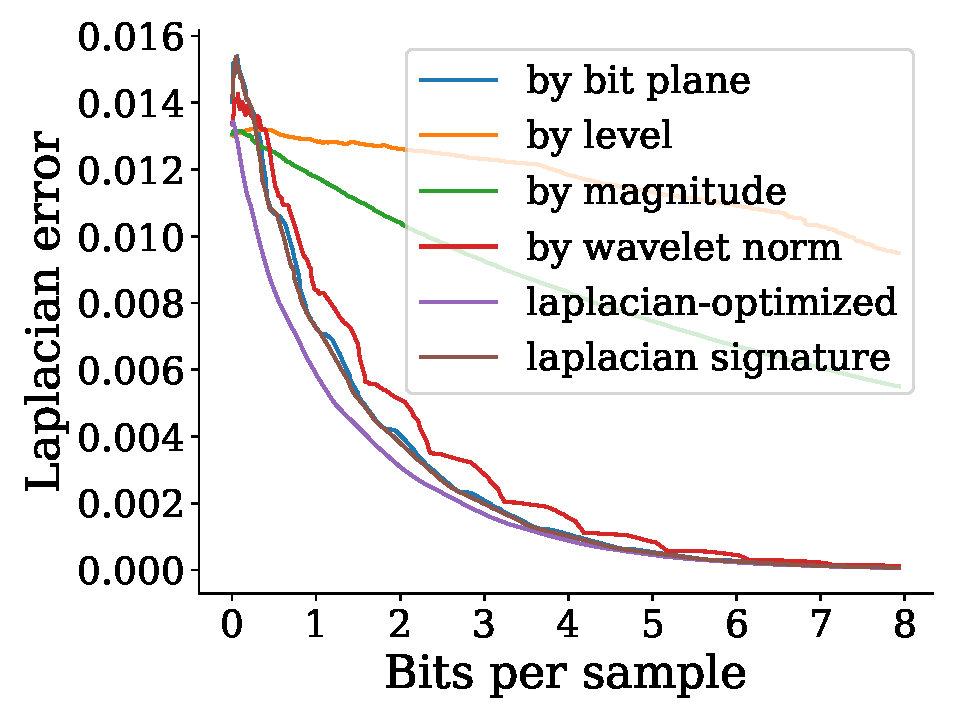
\includegraphics[width=0.24\linewidth]{laplacian/laplacian-optimized-boiler}}
\subcaptionbox{\emph{diffusivity}}
{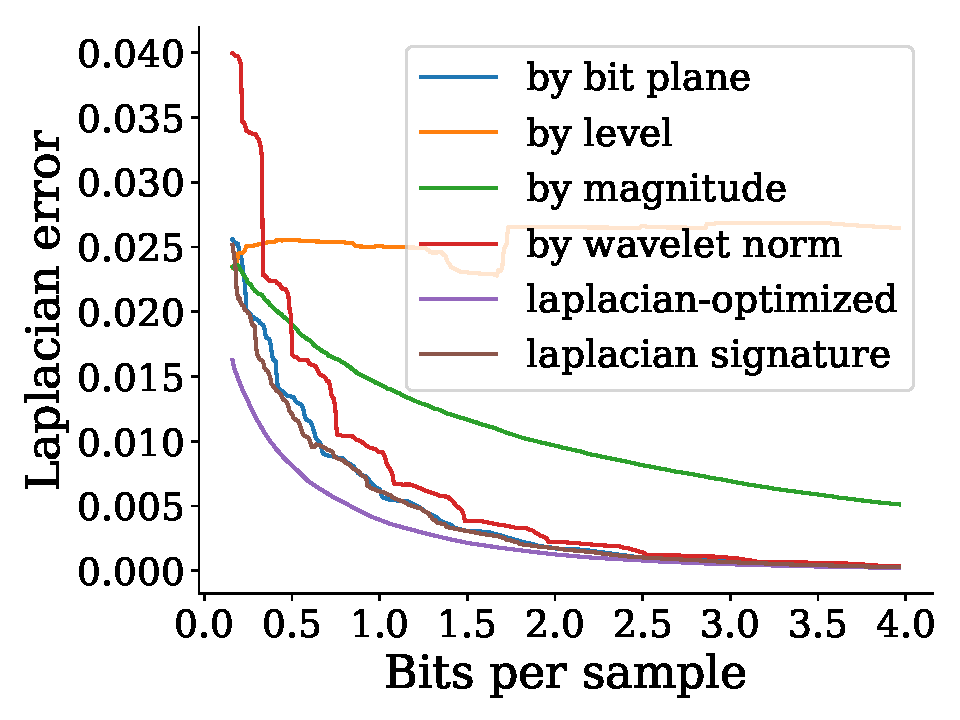
\includegraphics[width=0.24\linewidth]{laplacian/laplacian-optimized-diffusivity}}
\subcaptionbox{\emph{turbulence}}
{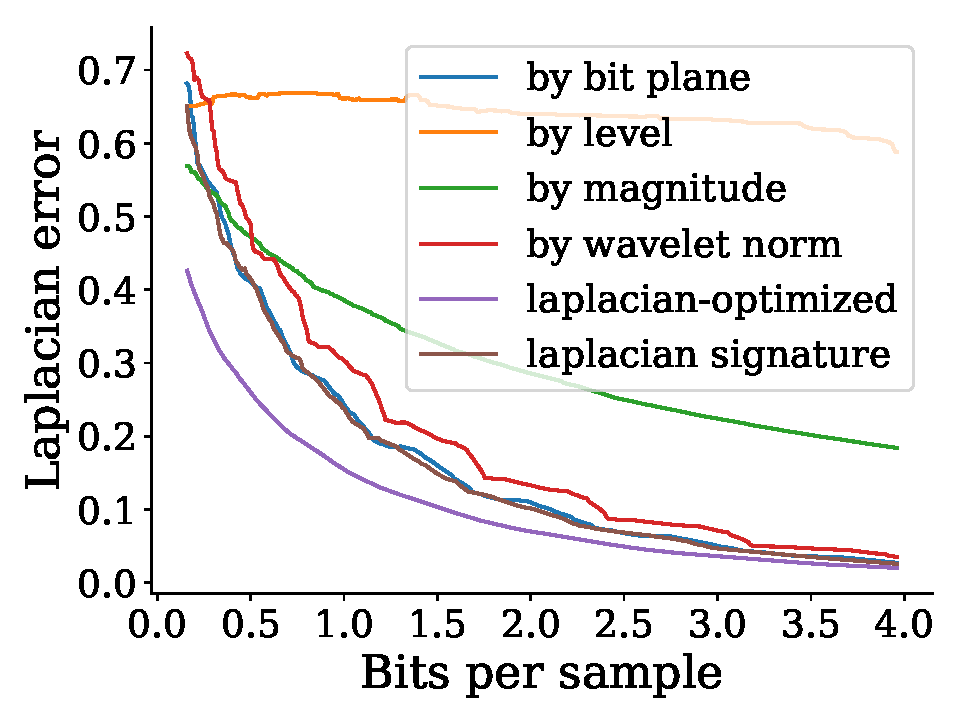
\includegraphics[width=0.24\linewidth]{laplacian/laplacian-optimized-turbulence}}
\subcaptionbox{\emph{pressure}}
{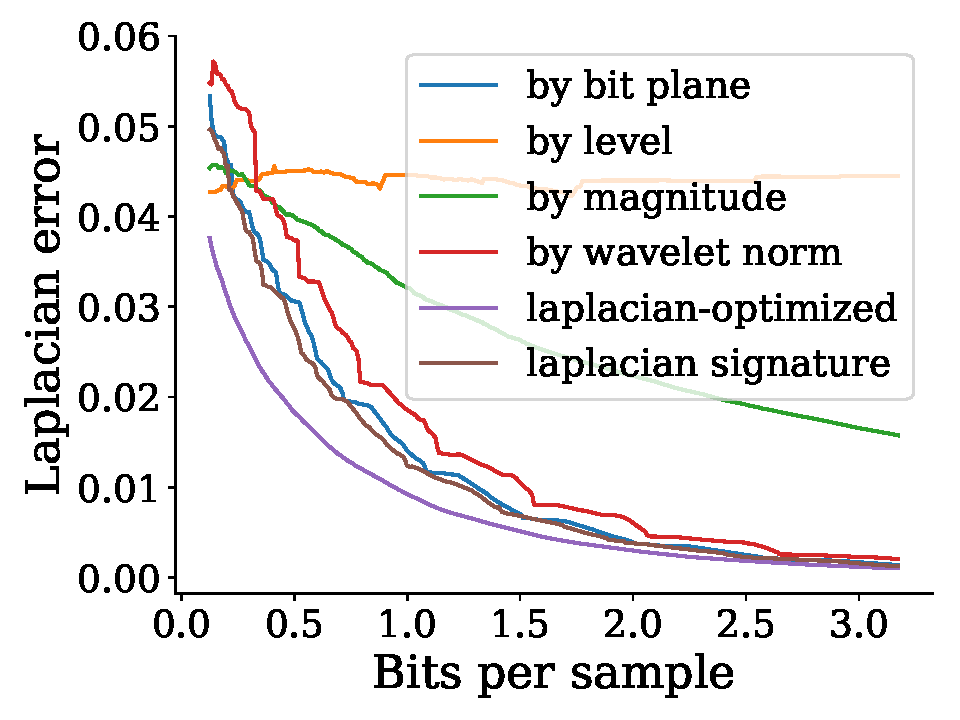
\includegraphics[width=0.24\linewidth]{laplacian/laplacian-optimized-pressure}}
\caption{Laplacian error comparison among streams. The plots are truncated to better highlight
differences without discarding important information. In all cases, in terms of error, $\slop <
\slsg < \sbit < \swav < \smag < \slvl$.}
\label{fig:laplacian-error-comparison}
\end{figure*}

\begin{figure*}[t]
        \centering
        \subcaptionbox{\emph{boiler}}
        {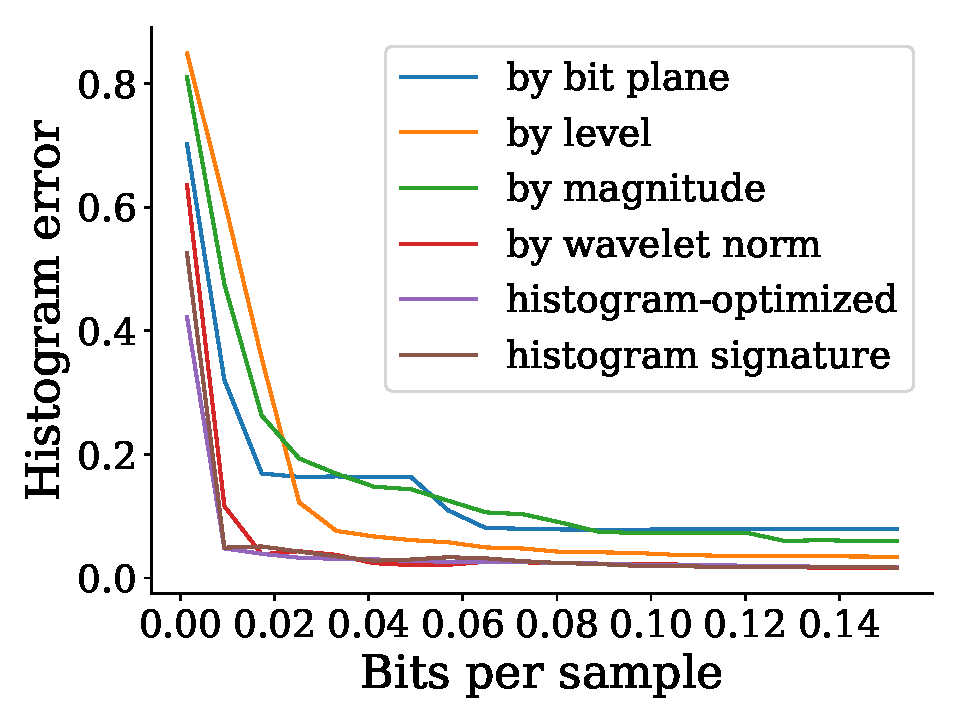
\includegraphics[width=0.24\linewidth]{histogram/histogram-optimized-boiler}}
        \subcaptionbox{\emph{diffusivity}}
        {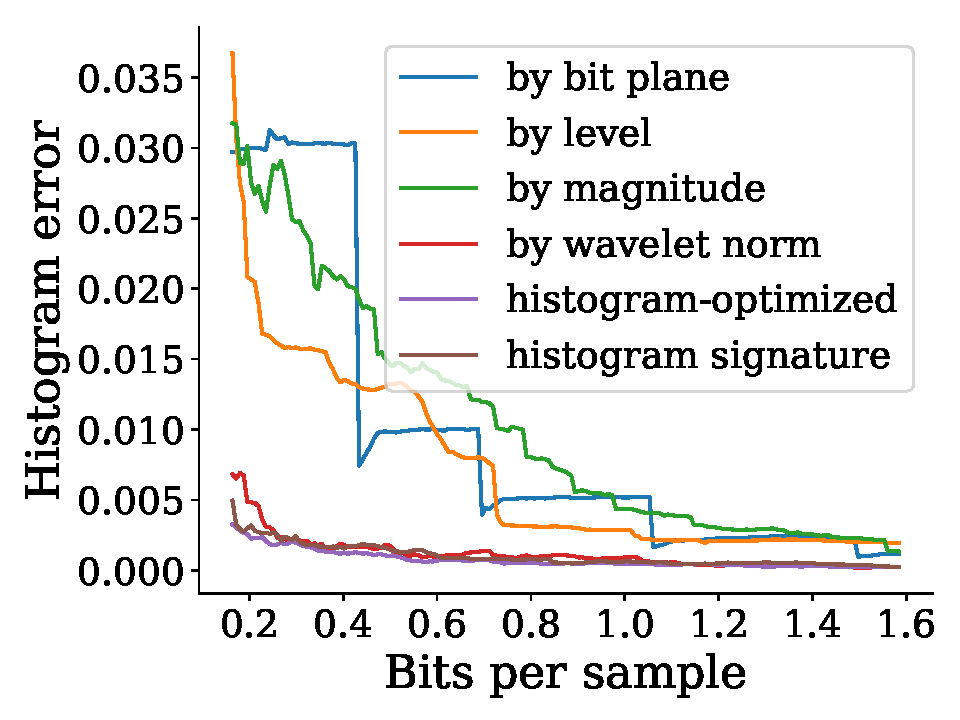
\includegraphics[width=0.24\linewidth]{histogram/histogram-optimized-diffusivity}}
        \subcaptionbox{\emph{kingsnake}}
        {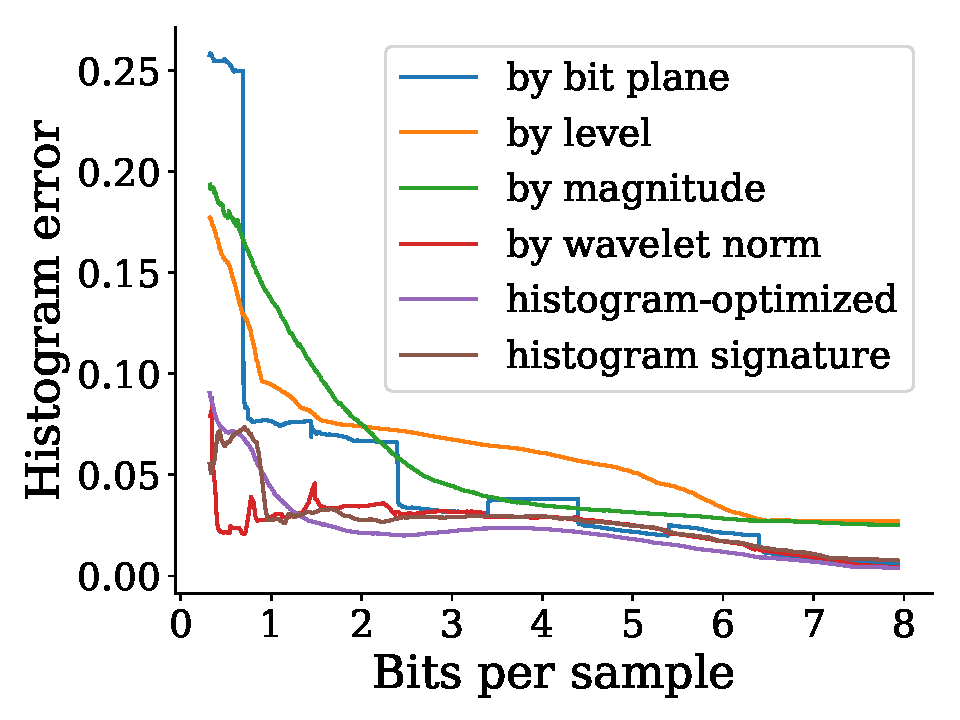
\includegraphics[width=0.24\linewidth]{histogram/histogram-optimized-kingsnake}}
        \subcaptionbox{\emph{foam}}
        {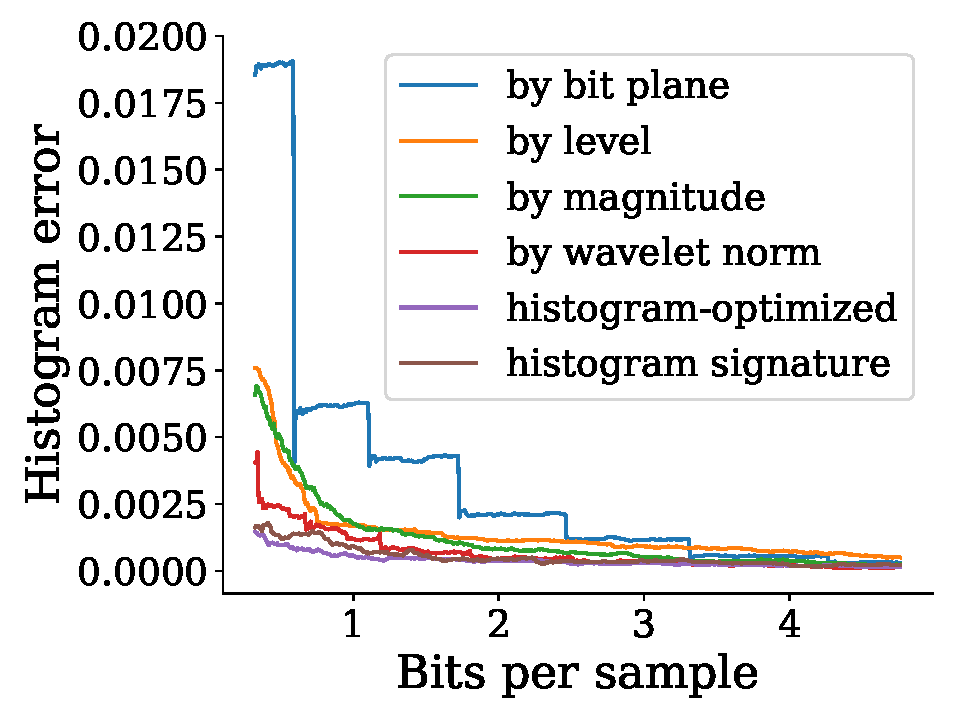
\includegraphics[width=0.24\linewidth]{histogram/histogram-optimized-foam}}
        \caption{Comparison of histogram errors among streams. Plots are truncated to highlight
        differences without hiding important trends. In general, in terms of error, $\shop \approx \shsg
        \approx \swav < \slvl, \sbit, \smag$. The erratic behavior at the beginning for \emph{kingsnake}
        is likely due to the data being too noisy. The especially poor performances of \sbit for
        \emph{boiler} and \emph{foam} are due to the ``shifting'' effect explained in~\Cref{sec:gradient}.
        Crossover points between \sbit and \slvl are explained in~\Cref{fig:histogram-explain}.}
        \label{fig:histogram-stream-comparison}
\vspace{1em}

        \centering
        \subcaptionbox{\emph{by level} (\slvl)}{
        {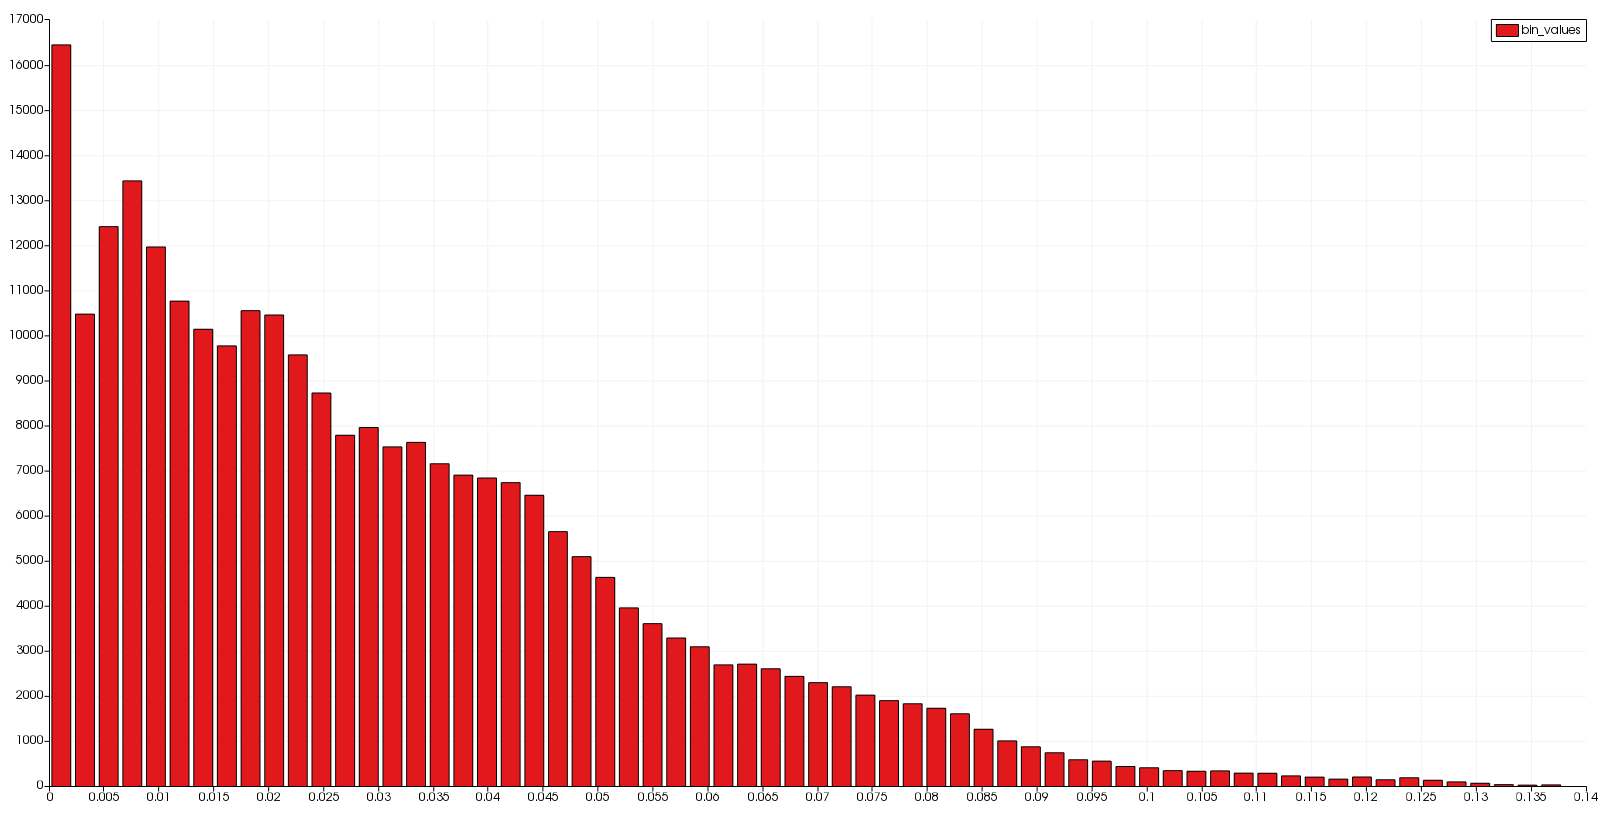
\includegraphics[width=0.155\linewidth]{histogram/histogram-boiler-level}}}
        \subcaptionbox{\emph{by bit plane} (\sbit)}{
        {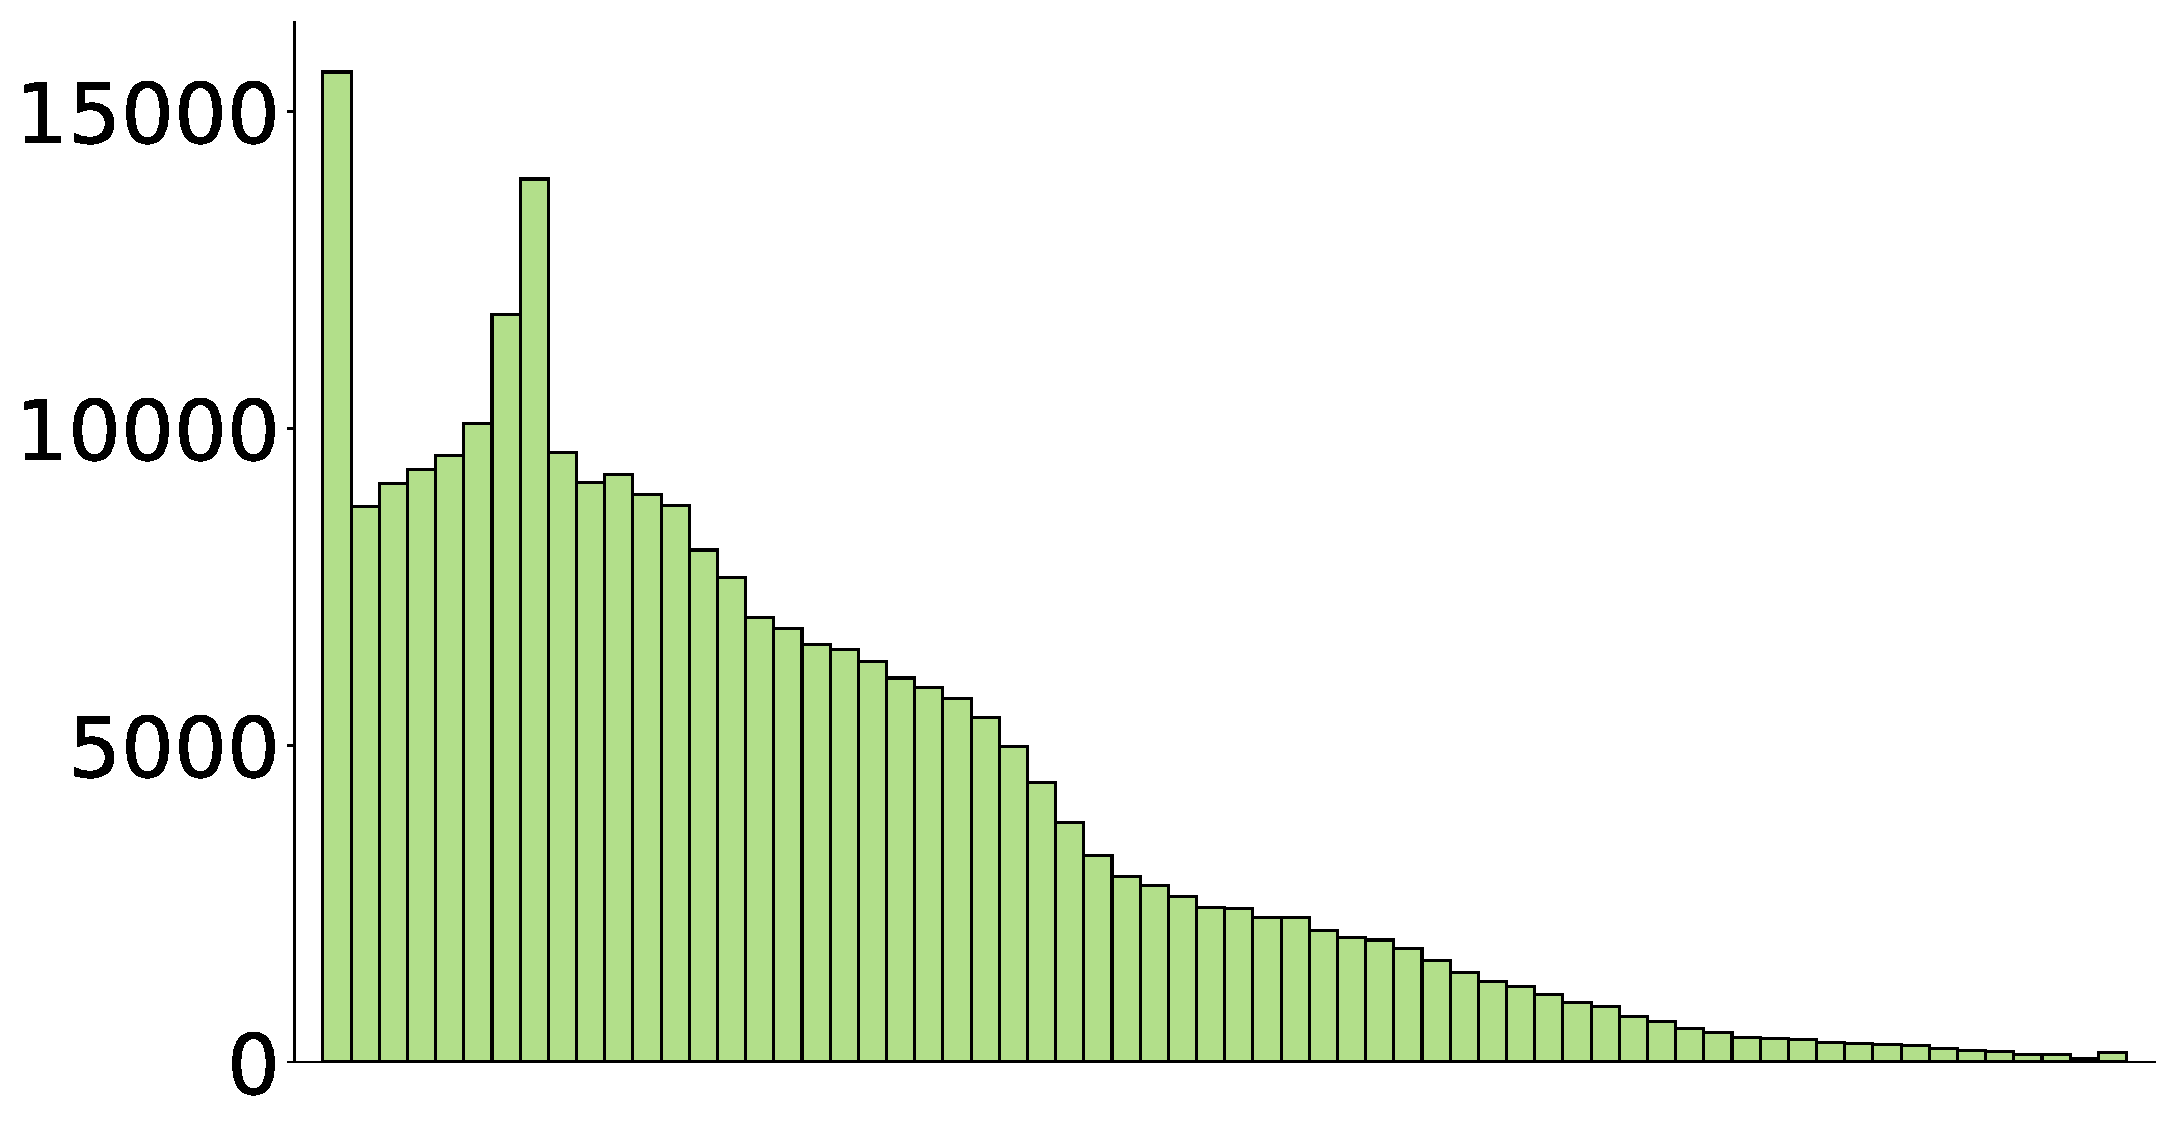
\includegraphics[width=0.155\linewidth]{histogram/histogram-boiler-bit-plane}}}
        \subcaptionbox{\emph{by magnitude} (\smag)}{
        {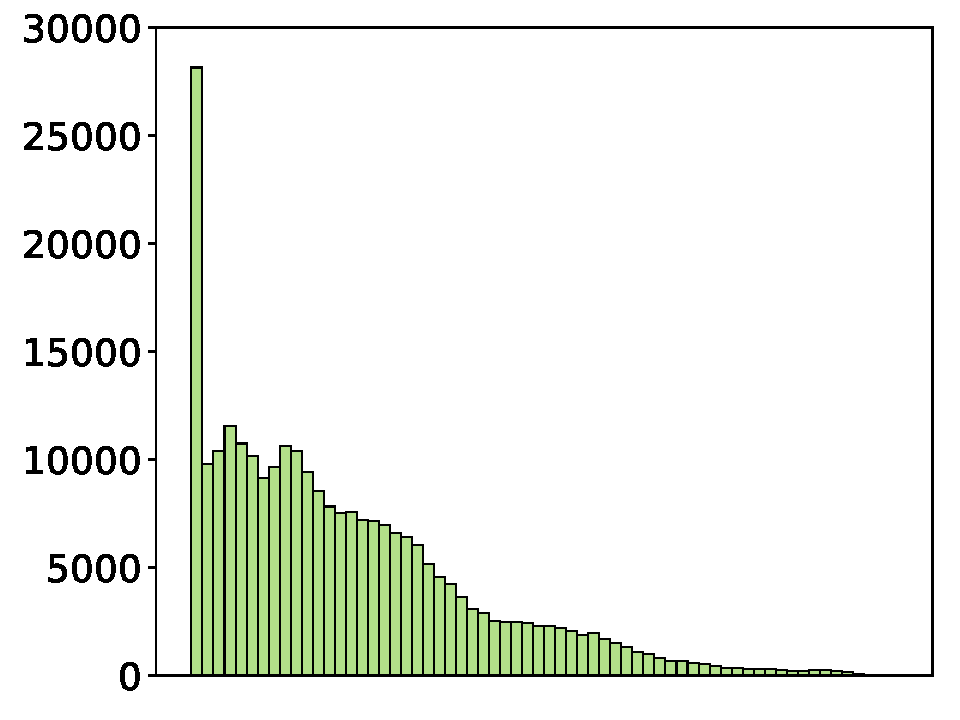
\includegraphics[width=0.155\linewidth]{histogram/histogram-boiler-magnitude}}}
        \subcaptionbox{\emph{by wavelet norm} (\swav)}{
        {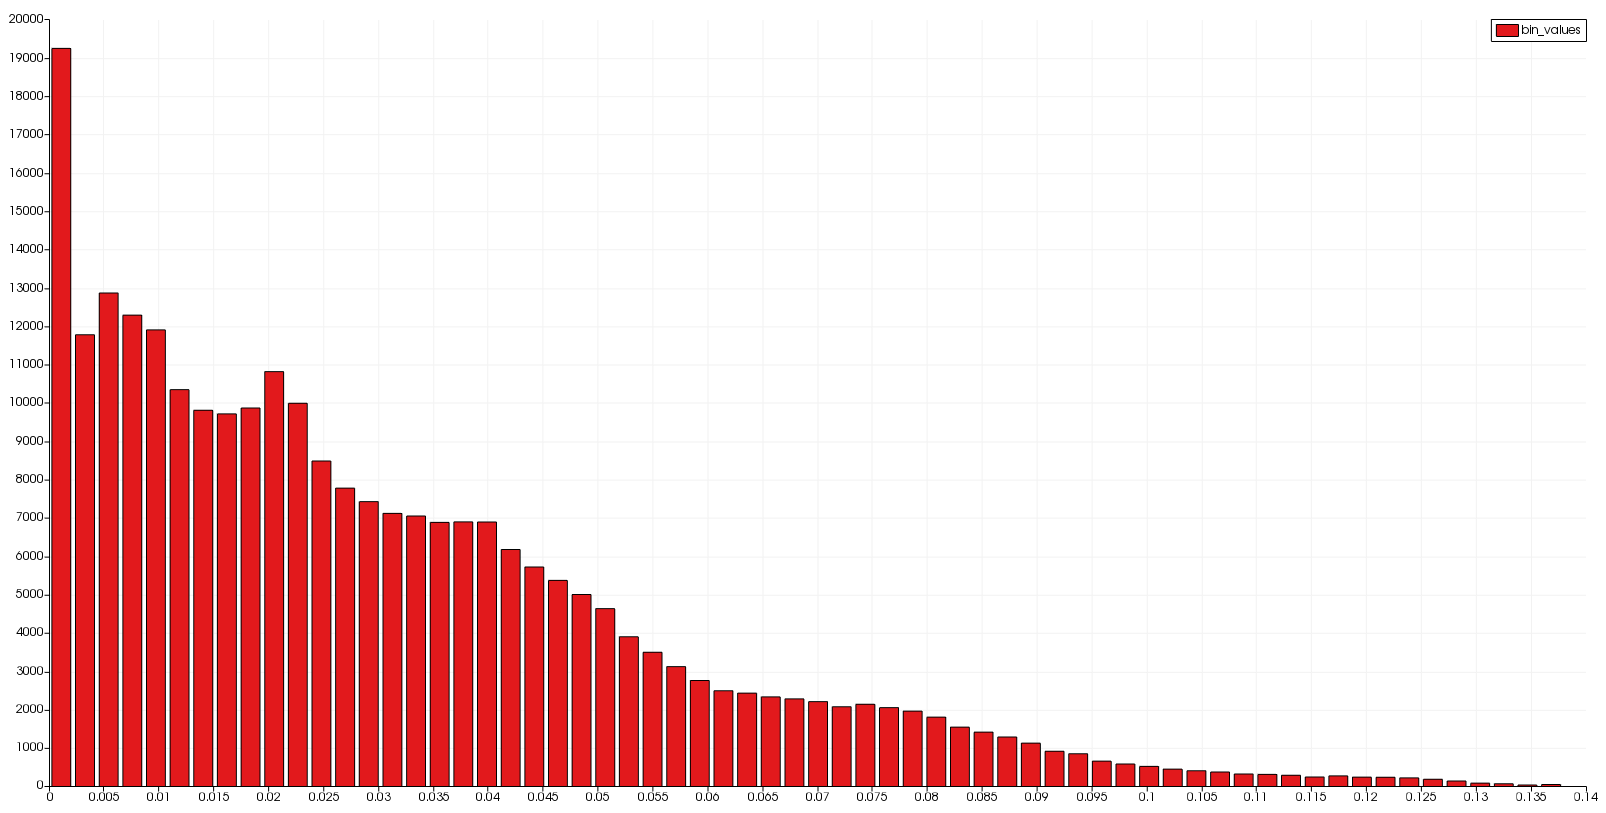
\includegraphics[width=0.155\linewidth]{histogram/histogram-boiler-wavelet-norm}}}
        \subcaptionbox{\emph{by signature} (\shsg)}{
        {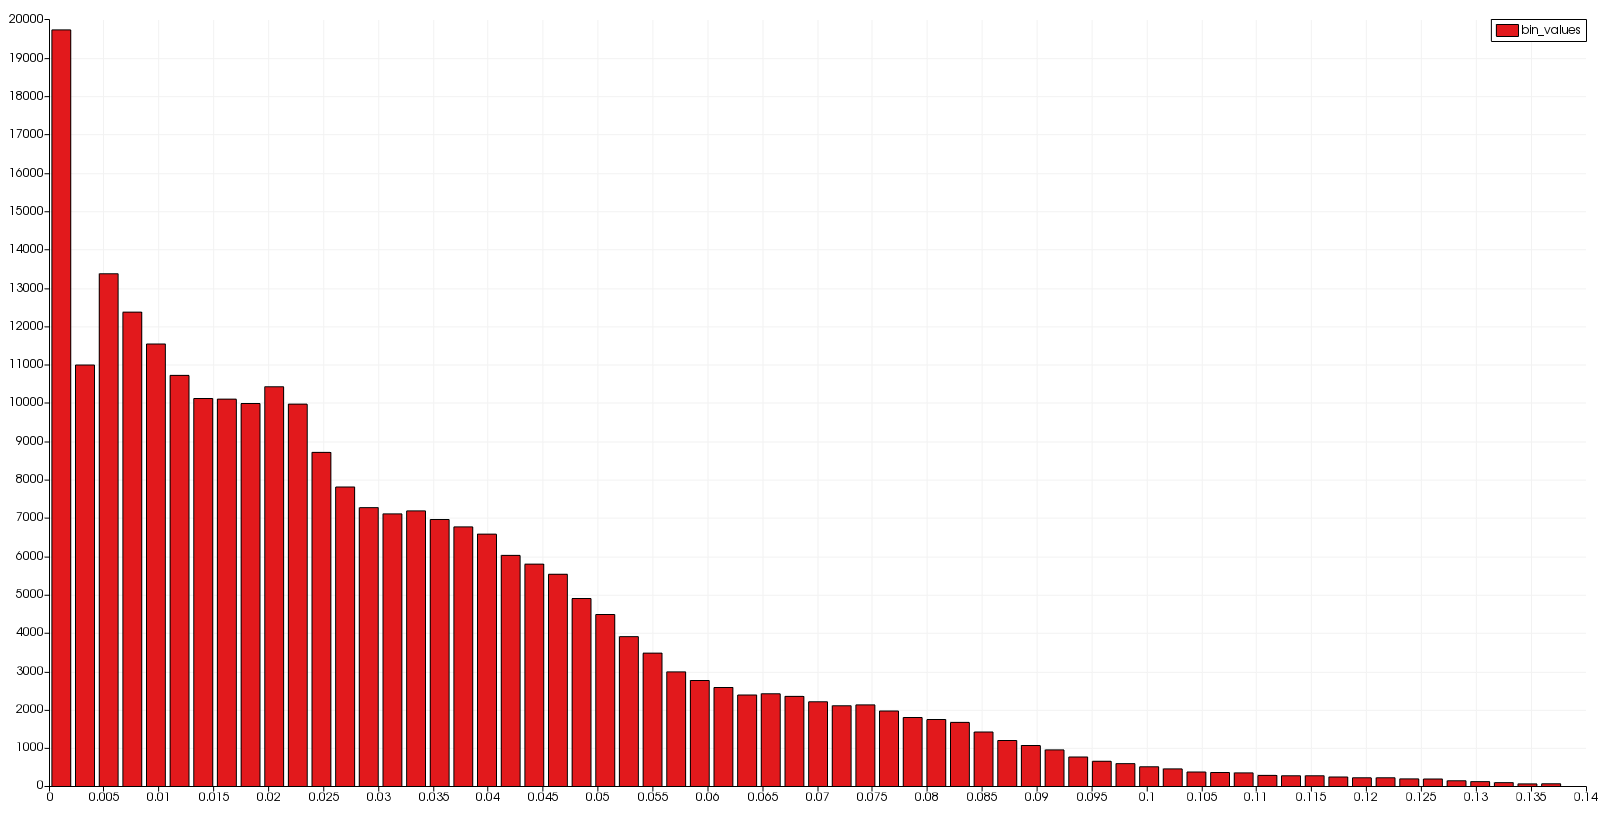
\includegraphics[width=0.155\linewidth]{histogram/histogram-boiler-signature}}}
        \subcaptionbox{\emph{reference}}{
        {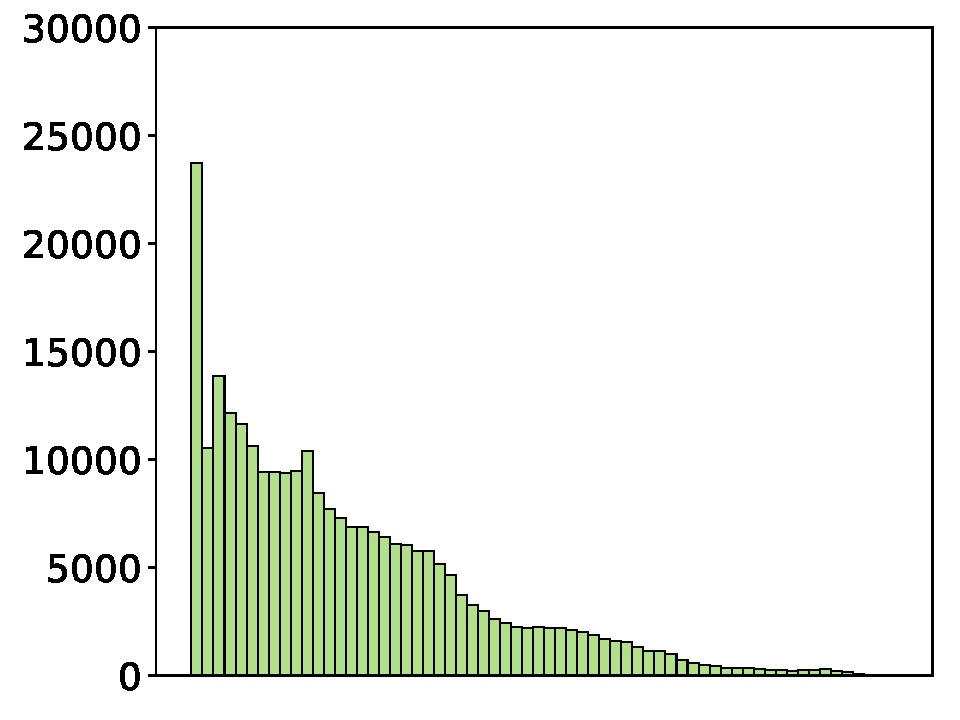
\includegraphics[width=0.155\linewidth]{histogram/histogram-boiler-groundtruth}}}
        \caption{Histograms of the \emph{boiler} data set, reconstructed at 0.13 bps. \slvl, \swav, and
        \shsg produce histograms that share a shape similar to the reference histogram, with most of the
        peaks and valleys preserved. In contrast, \sbit produces a spurious peak not found in the
        reference. Finally, \smag's histogram has a widely skewed distribution where too many values fall
        into the first bin.}
        \label{fig:histograms-boiler}
        \vspace{-1em}
\end{figure*}

\subsubsection{Gradient Computation} \label{sec:gradient}

Given a function $f$ defined on a grid, its gradient at a grid point \mbox{$\x = (x,y,z)$} is the
vector $\nabla f(\x) = \left(\frac{\partial f}{\partial x}, \frac{\partial f}{\partial y},
\frac{\partial f}{\partial z}\right)$. We use a five-point stencil to compute the gradient, i.e.,
$\frac{\partial f}{\partial x} \approx \frac{1}{12}f(x-2,y,z) - \frac{2}{3}f(x-1,y,z) +
\frac{2}{3}f(x+1,y,z) - \frac{1}{12}f(x+2,y,z)$. The error between a gradient field $\nabla f$, and
its low-bit-rate approximation $\nabla
\tilde{f}$, is defined as $\err(\nabla \tilde{f}, \nabla f) = \sqrt{\frac{1}{N}
\sum_{i=1}^{N}{\norm{\nabla \tilde{f}(\x_i)-\nabla f(\x_i)}^2}}$. Using~\Cref{alg:greedy}, we
compute a \emph{gradient-optimized} stream, \sgop, i.e., a stream that minimizes the difference
between the reconstructed gradient field and the original gradient field.

\Cref{fig:gradient-error-comparison} shows the gradient error incurred by different streams for four
data sets. In general, we observe the ordering of performance (from best to worst) as: \sgop, \sgsg,
\sbit, \swav, \smag, \slvl. This ordering can also be seen in~\Cref{fig:gradient-rendering-diff},
where the $x$-component of the gradient field for \emph{tuburlence} is rendered at 0.5 bps. Unlike
the RMSE case, \sbit produces better approximations of the gradient field compared to \swav.

We further investigate this difference by extracting a 1D line from the \emph{plasma} data set and
reconstructing the function using \sbit and \swav at 0.6 bps
(\Cref{fig:bit-plane-vs-wavelet-norm-gradient}). Because the coarse-scale coefficients in \sbit are
approximated at low precision, the reconstruction from \sbit is inaccurate in areas of low
gradients. In contrast, \swav's reconstruction is accurate in low-gradient areas, but lacks the
resolution to resolve the high-gradient areas, because \swav frequently intersperses bits that
improve resolution with bits that improve precision, unlike \sbit, which always streams bits that
improve resolution first. Therefore, \swav tends to produce a ``smoother'' reconstruction that
\emph{on average} (e.g., in terms of RMSE) is close to the original function. \sbit, on the other
hand, tends to capture well the function's shape (due to fine-scale bits), but the whole function
can be ``shifted'' slightly due to the lack of precision in coarse-scale coefficients. However, the
error caused by this shifting reduces significantly when taking the gradient, which cancels any
constant shift. \sbit, therefore, works better than \swav for gradient computation, because it is
better able to retain sharp features.



\begin{figure}[!b]
\centering
\subcaptionbox{\emph{by bit plane} (\sbit)}{
{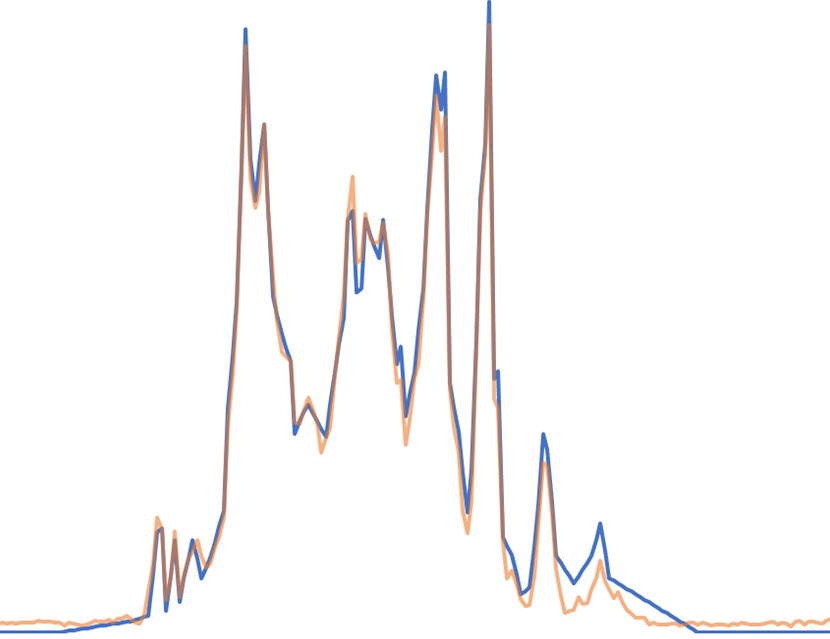
\includegraphics[width=0.48\linewidth]{gradient/gradient-bit-plane}}} 
\subcaptionbox{\emph{by wavelet norm} (\swav)}{
{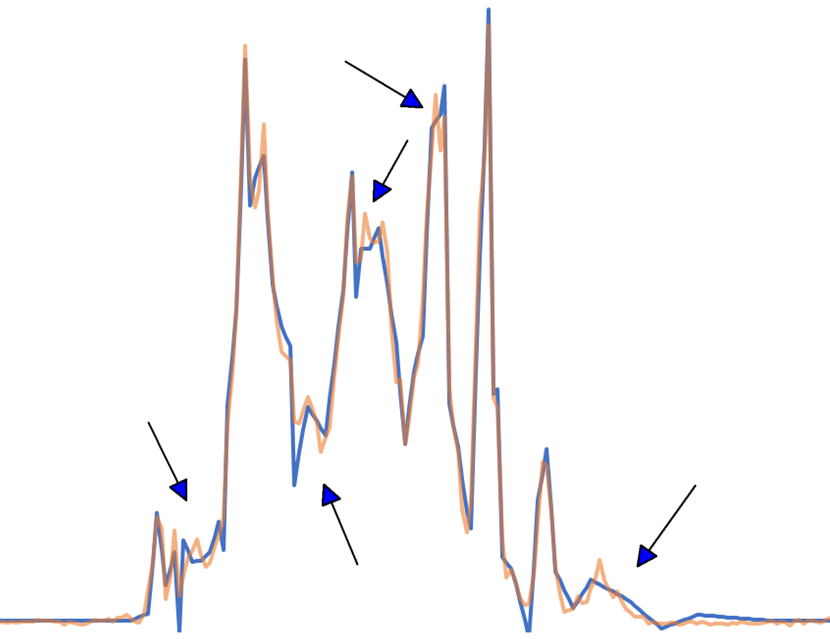
\includegraphics[width=0.48\linewidth]{gradient/gradient-wavelet-norm}}}
\caption{A 1D line extracted from \emph{plasma}, and reconstructed using \sbit and \swav at 0.6 bps.
The original data is in orange and the reconstructions are in blue. \swav captures well the function
values in low-gradient regions, where \sbit struggles (red arrows). However, \sbit retains the shape
of the original function well in areas of both low and high gradients, where \swav instead produces
smooth approximations (blue arrows). \sbit therefore is better for derivative computations, where a
function's shape (or its relative values) matters more than its absolute values.}
\label{fig:bit-plane-vs-wavelet-norm-gradient}
\vspace{-1em}
\end{figure}



\sgop again outperforms the rest of the streams. \slvl and \smag perform poorly for gradient
computation, lacking the resolution to capture sharp features. \sgsg closely follows \sbit in
performance (it is slightly better than \sbit for \emph{boiler} at very low bit rates). These
results suggest that while \swav is the best among the data-independent streams when optimizing for
RMSE, \sbit is better for gradient computation.



\subsubsection{Laplacian Computation}\label{sec:laplacian}

The Laplace operator is a second-order differential operator defined as the divergence of the
gradient field. The Laplacian of a 3D field is defined as $\Delta f = 
\frac{{\partial}^2}{\partial{x^2}}f+\frac{{\partial}^2}{\partial{y^2}}f+\frac{{\partial}^2}{\partial{z^2}}f$.
%
Using a five-point finite difference, we approximate 
%$\frac{{\partial}^2}{\partial{x^2}}f(x,y,z)
$\frac{{\partial}^2 f}{\partial{x^2}}
\approx
-\frac{1}{12}f(x-2,y,z)+\frac{4}{3}f(x-1,y,z)-\frac{5}{2}f(x,y,z)+\frac{4}{3}f(x+1,y,z)-\frac{1}{12}f(x+2,y,z)$.
We use the root-mean-square error to compare two Laplacian fields, i.e., $\err(\Delta
\tilde{f},\Delta f)=\text{RMSE}(\Delta \tilde{f},\Delta f)$. As usual, we use~\Cref{alg:greedy} to
compute a \emph{Laplacian-optimized} stream, \slop, which minimizes $\err$, and an \slsg stream from
its signature.~\Cref{fig:laplacian-error-comparison} plots the error curves for all relevant
streams. The plots here largely follow the ones in~\Cref{fig:gradient-error-comparison}, in terms of
relative performance among the streams, but with more discernible gaps between \sbit and \slsg.



